\paragraph*{Evolution in vitro of ribosome activities}
The group of Szostak was also able to develop some in vitro selection systems
that led to the evolution in vitro of ribosome with real enzymatic activity.
After 10 cycles of evolution the activity increased more that 2.5 million fold.

\section{Prokaryoutes and Eukaryotes}
Biological organisms can be "Prokaryoutes" or "Eukaryoutes". Procaryotes are
bacteria and archea. They are unicellular organisms with a simple structure,
without internal compartments. Eukaryoutes are more complex. Very often they are
multi-cellular organism. They include plants, animals but also many unicellular
organisms (yeast, protozoa and many other). Eukaryotes cells have different
compartments delimited by internal membranes such as nucleus, mitochondria,
endoplasmic reticulum and Goldi Apparatus. During cellular division, the DNA
of Eukaryotes becomes condensed and forms chromosomes that are "chromo" because
they become easily coloured with basic dyes and are visible under the
microscope.

\paragraph*{Prokaryotes} Prokaryotes are very simple. While the size of a
bacterium is about 1 um, a typical Eukaryotic cell is 10-20 times bigger.

Both Prokaryotes and Eukaryotes exchange their genetic information (DNA)
among individuals of the same species. Prokaryots have a simple system to
transfer some segments of DNA through a "sex pilus" from one individual to
another, but they exchange DNA mainly in critical conditions, otherwise they
duplicate as clones.

\paragraph*{Haploid and diploid}
Be diploid allows you to accumulate faulty genes.

\begin{figure}[H]
  \centering
  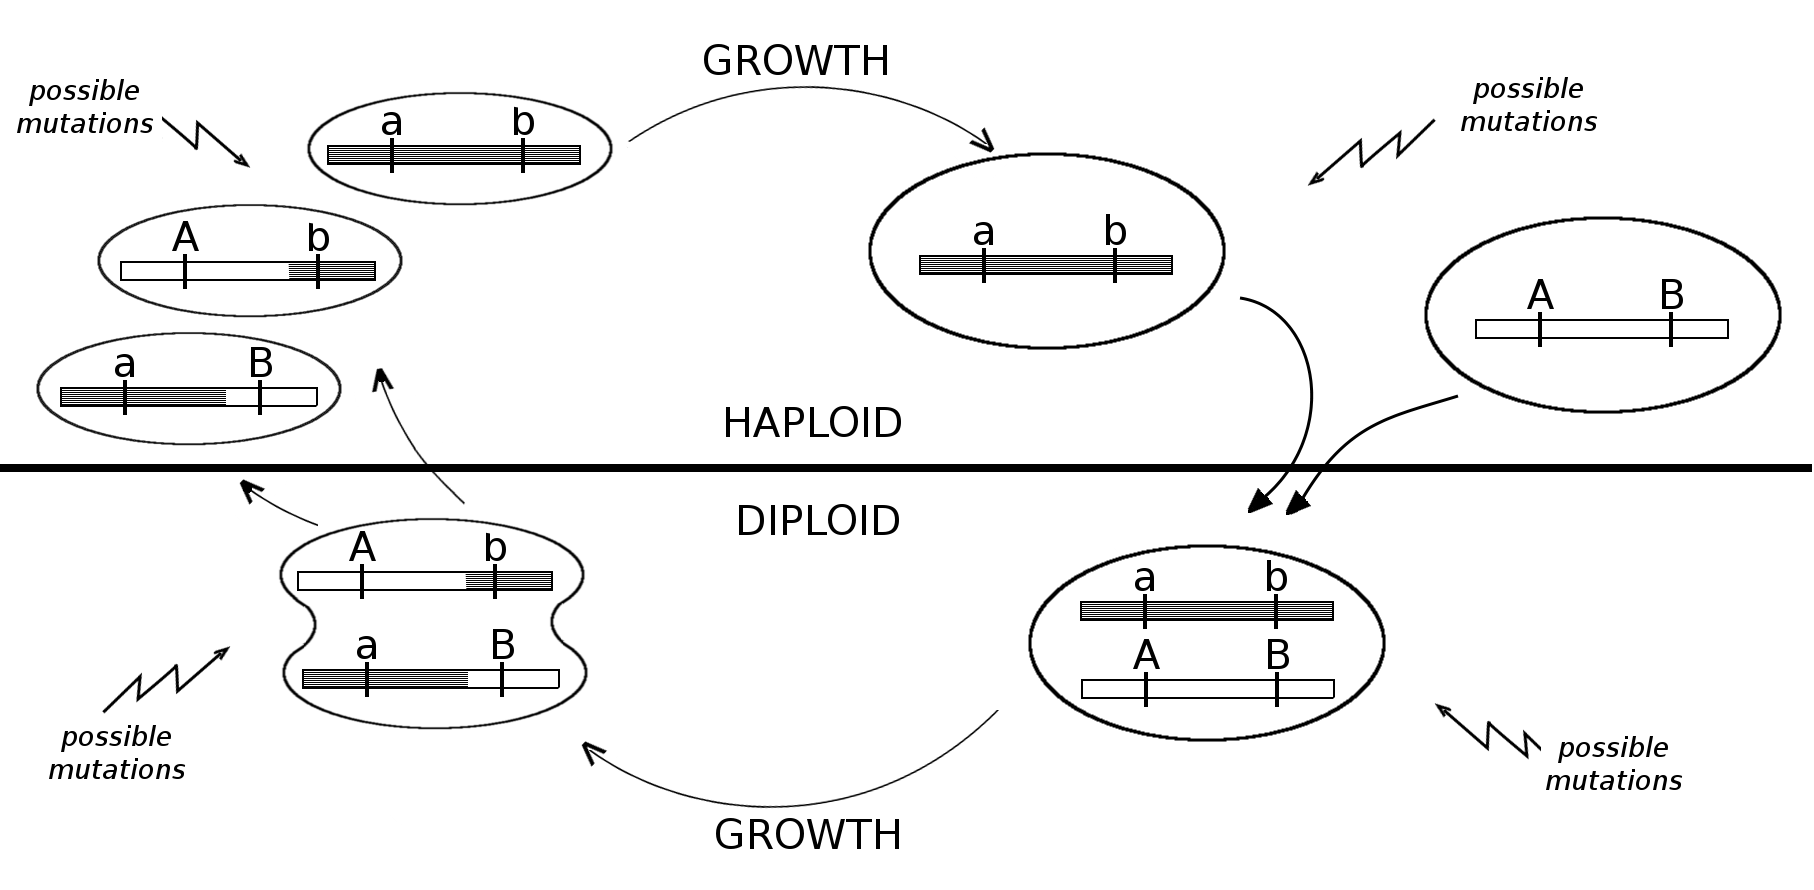
\includegraphics[scale=0.5]{life_cycle}
\end{figure}

During cellular division, the DNA of Eukaryots becomes condensed and forms
chromosomes. Typically Eukaryotes have sexual reproduction that implies some
alternation between haploid and diploid stages. In Eukaryotes, FERTILIZATION
occurs when two haploid cells merge and become one diploid cell. Usually, in a
multi-cellular organism the diploid cells duplicate by MITOSIS; thus a
multi-cellular organism is typically made by many diploid cells with the same
genomics DNA. MEIOSIS occurs when a diploid cell produces haploid cells, often
called "gametes". During meiosis a process called "CROSSING OVER" occurs,
resulting in the exchange of parts between homologous chromosomes. In human,
the probability that a crossing over occurs within any two loci at a distance
of 1 million bases is about 1\% per generation. In other organisms may occur
with different frequency. The crossing over, per se, does not produce mutations
but allows the mix of the genetic diversity present in the two parents. Genetic
diversity is fundamental for evolution. Being diploid allows to maintain a much
larger pool of variant genes, most of these mutated genes do not work as well
as the original, but together with other mutations may improve the fitness.
Some organisms, for instance yeast, have very similar haploid and diploid
cells. Most multi-cellular organisms have a very predominant part of their life
cycle as diploid. The question is: "Why diploid seems to be better?" and "Why
complex organisms (plants and animals) are diploid?"

\paragraph*{Saccharomyces cerevisiae}
First eukaryotic genome that has been sequenced (1996). It's 13 billion bases
with 6000 genes.

\paragraph*{Caenorhabditis elegans}
First animal genome that has been sequenced (1998), 100 billion bases.
